\documentclass{ctexart}
\usepackage{amsmath}
\usepackage{float}
\usepackage{amssymb}
\usepackage{graphicx}
\usepackage{gbt7714}
\usepackage{pifont}
\usepackage{wrapfig}
\usepackage{multirow}
\ctexset{
    % 修改 section。
    section={   
        name={,、},
        number={\chinese{section}}
    }
}

\title{双棱镜干涉现象和激光波长的测量}
\author{陆知辰-10225301478}
\date{\today}
\graphicspath{{figure/}}

\begin{document}

\begin{titlepage}
  \centering
  % 插入图片
  
\includegraphics[width=0.5\textwidth]{ecnu.png}
  
  % 空行用于调整标题位置
  \vspace*{\baselineskip}
  
  % 标题
  \Huge\textbf{物\quad 理\quad 实\quad 验 \quad (二)}
  % 空行用于调整标题和其他信息之间的间距
  \vspace*{0.3\baselineskip}
  
  % 具体实验名称
  \huge 双棱镜干涉现象和激光波长的测量
  
  % 空行用于调整时间和其他信息之间的间距
  \vspace*{2\baselineskip}
  
  % 时间
  \large 时间:\today
  
  % 空行用于调整时间和其他信息之间的间距
  \vspace*{\baselineskip}
  
  % 创作人
  \large 创作人:陆知辰
  
  % 空行用于调整创作人和学号之间的间距
  \vspace*{\baselineskip}
  
  % 学号
  \large 学号:10225301478
  
\end{titlepage}
\newpage
\tableofcontents
\newpage
\section{实验摘要}
  \subsection{实验概要}
  光的干涉现象是光波动说的基础,产生相干光有两类典型方法,
  具体为分振幅法和分波前法,非涅耳双棱镜干涉则属于分波前法,
  菲涅尔双棱镜干涉实验曾在历史上为确立光的波动学说起过重要作用,它提供了一种用简单仪器测量光的波长的方法.
  \subsection{实验目的}
  1.\quad 观察双棱镜光的干涉现象和特点。

  2.\quad 掌握获得双光束干涉的方法。进一步理解产生干涉的条件。
  
  3.\quad 掌握测量激光波长的实验原理和方法。

\section{实验原理}
双棱镜由两个楔角很小的直角棱镜组成,且两个棱镜的底边连在一起(实际上是在一块玻璃上,将其上表面加工成两块楔形板),
用它可实现分波前干涉.通过对其产生的干涉条纹间距的测量,可推算出光波波长。

如图\ref{guanglu}所示,双棱镜 AB的棱脊与过S的垂直平面平行,H为观察屏,且三者都与光具座垂直放置。
由光源发出的光,经透镜$L_{1}$,会聚于S点,
由S出射的光束投射到双棱镜上,经过折射后形成两束光。这两束光好像是从虚光源$S_{1}$和$S_{2}$发出的在相互重叠的区域内产生干涉。
我们可在观察屏上看到明暗交替的、
等间距的直条纹。中心O处因两束光的光程差为零而形成中央亮纹,其余的各级条纹则分别排列在中央亮纹的两侧。
从这个过程看,双棱镜干涉相当于以$S_{1}$和$S_{2}$为双孔的杨氏干涉。

\begin{figure}[H]
  \centering
  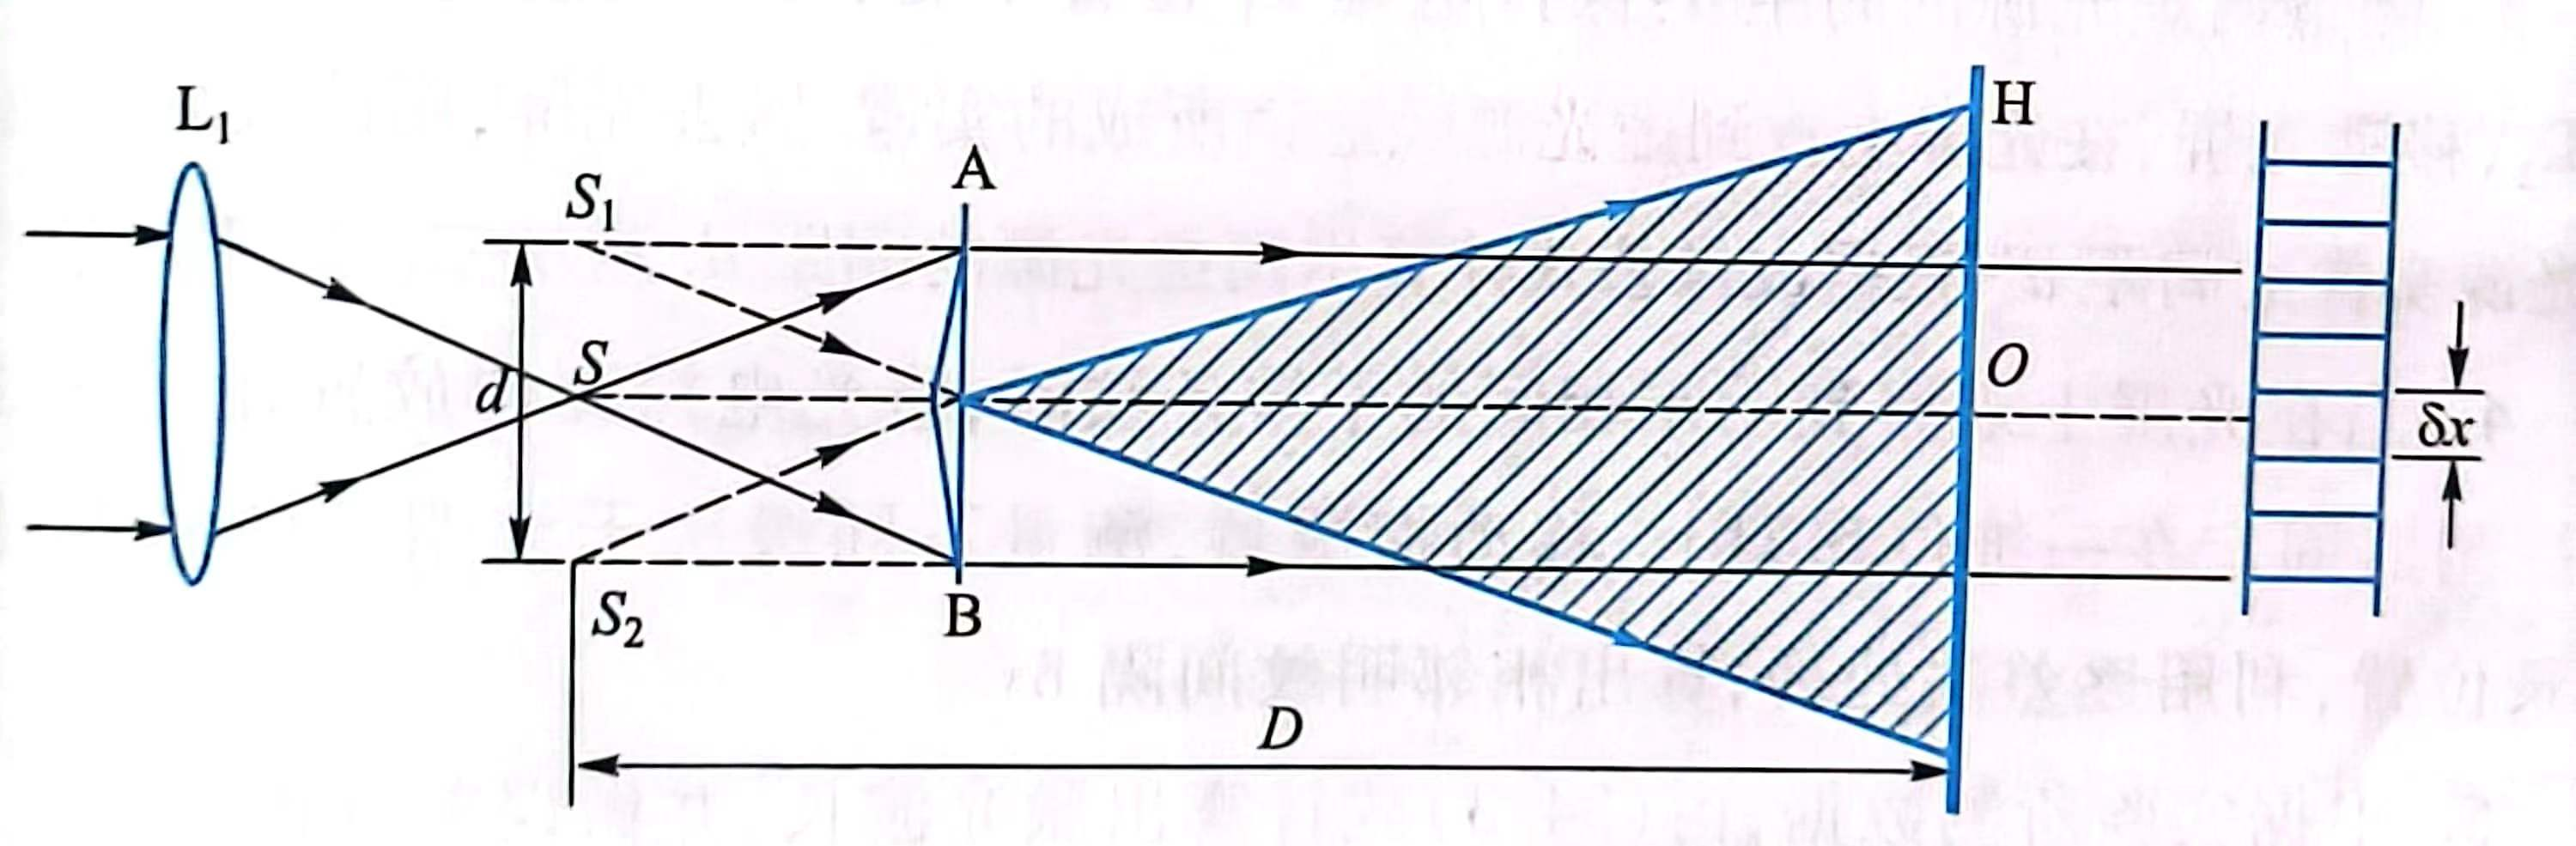
\includegraphics[height=0.5\textheight,width=0.8\textwidth]{guanglu.jpg}
  \caption{双棱镜干涉光路图}\label{guanglu}
\end{figure}

设两虚光源$S_{1}$和$S_{2}$间的距离为d,虚光源平面S的中心到屏的中心,之间的距离为D;又设H屏上第k(k为整数)级亮纹与中心O相距为$x_{k}$,当$x_{k}<D,d<<D$时
干涉亮纹的位置$x_{k}$由下式决定

\begin{equation}
  x_{k}=\frac{D}{d} k \lambda
\end{equation}

同样,暗纹的位置$x_{k}^{'}$可以写为

\begin{equation}
  x_{k}^{'}=\frac{D}{d} (k+\frac{1}{2}) \lambda
\end{equation}

则任意两相邻的亮纹(或暗纹)之间的距离为

\begin{equation}\label{deltax}
  \delta x = x_{k+1} - x_{k} = \frac{D}{d} \lambda
\end{equation}

式\ref{deltax}表明,只要测出d、D和$\delta x$即可算出光波波长入,其中D可在实验上测得(透镜 L,的焦平面位置为虚光源的位置),
$\delta x$可由实验上的光电探测器描绘的光强随位移的变化关系求得.
d的值一般采用凸透镜将虚物成实像的方法获得.在本节的实验32中,介绍了凸透镜的成像公式法和两次成像法这两种方法,
利用成像公式法,虚物光点在屏上成像,测出像的宽度,基于相似三角形,就可以求出虚物的d值.利用两次成像法,测量得到虚物成大像和小像的宽度,两者相乘,就可以得到虚物的d值。

\section{实验装置器材介绍}
光学实验导轨,激光器,双棱镜,光电探头器,一维位移架,凸透镜等。

\section{实验内容及实验步骤}
1.按图\ref{guanglu}所示光路简图在光学实验导轨上按照顺序摆好各光学元件.

2.调节光路,使所有光学元件等高共轴。激光器输出的水平激光通过透镜工的中心,人射到双棱镜的脊上,
在光屏上可观察到明暗相间的干涉条纹。(注意:入射到双棱镜上的光斑应大一点,这样干涉条纹质量较高。

3.测量两虚光源的间距d:保持透镜L,位置不变,在双棱镜与光屏之间放置透镜L,移动光屏,
在光屏上找到虚光源经透镜所成的实像.撤去光屏,用读数显微镜测得虚光源实像的间距$d^{'}$,根据成像公式计算出两虚光源的间距d.测量三次取平均值。

4.当在光屏上观察到明暗相间的干涉条纹时,将光电探测器放置在光屏处.光电探测器固定在一维位移架上,
移动探测器,测量不同级次干涉明纹的光强,同时记录位置,利用逐差法处理,算出相邻明纹间隔$\delta x$。

5.根据实验所测数据,由式\ref{deltax}计算出激光波长,并做误差分析。
\newpage

\section{实验原始数据}
\begin{figure}[H]
  \centering
  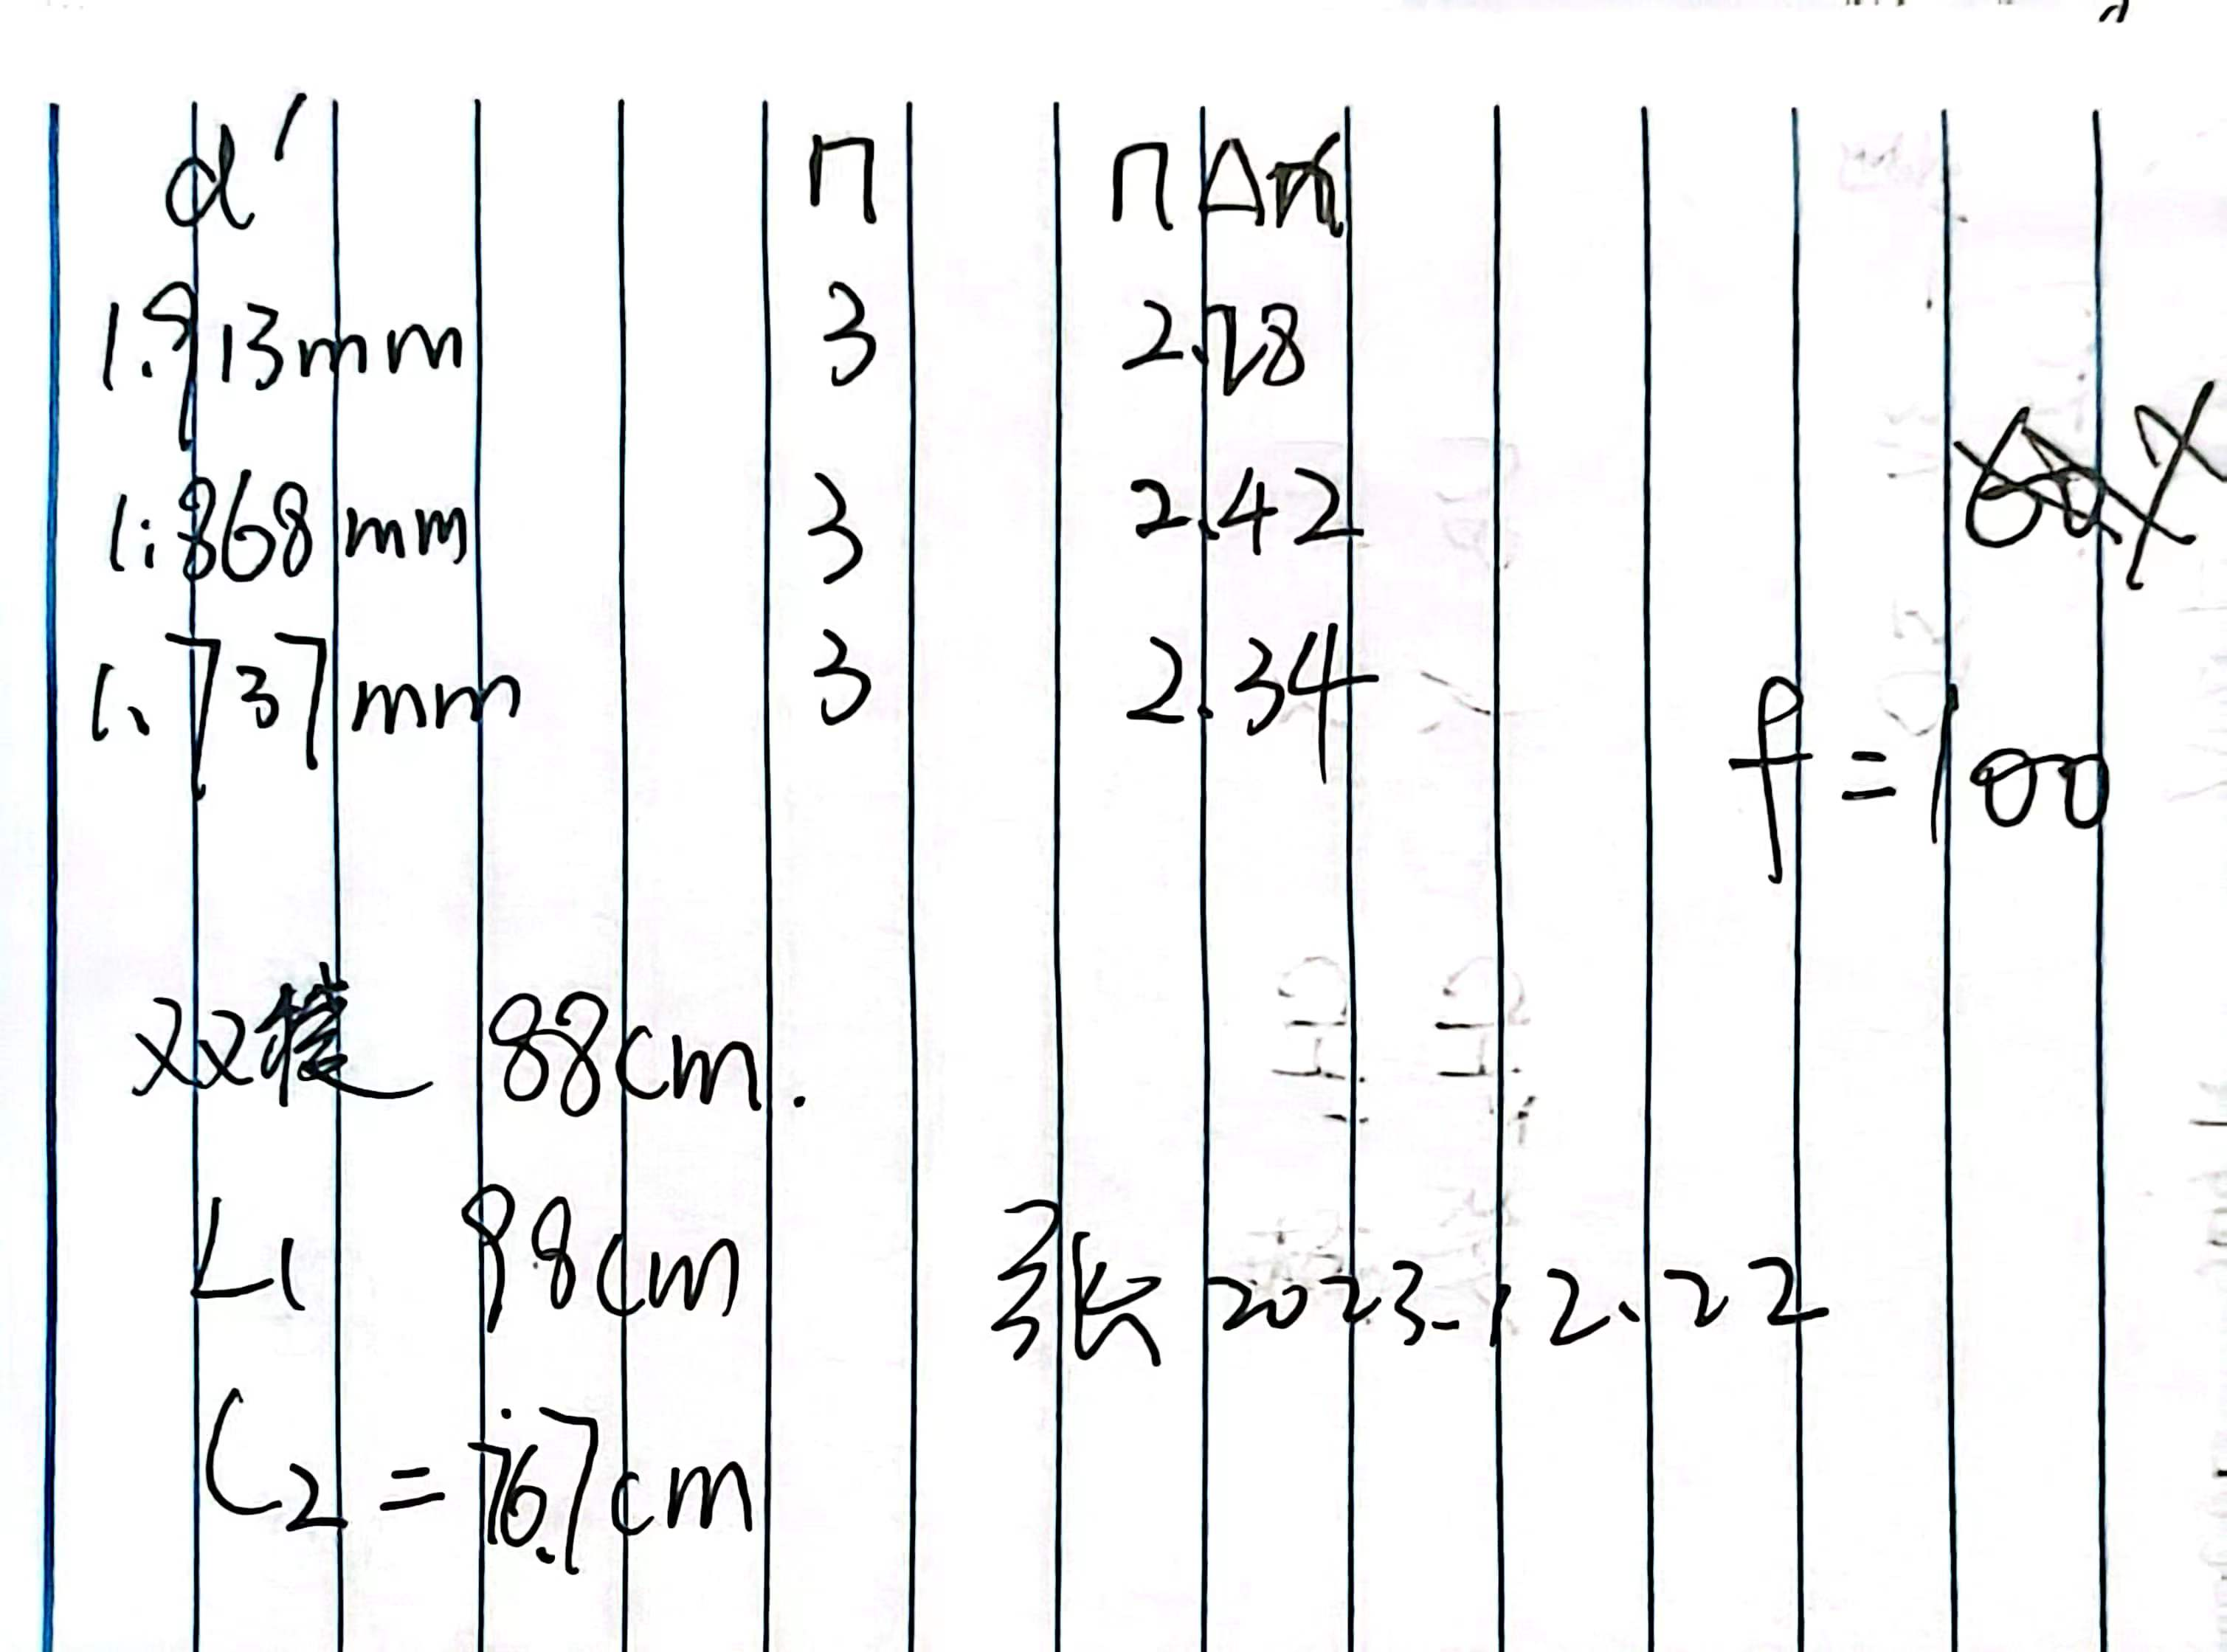
\includegraphics[height=0.5\textheight,width=1\textwidth]{yuanshishujv.jpg}
  \caption{实验原始数据}\label{yuanshishujv}
\end{figure}
\newpage

\section{实验数据处理}
  \subsection{计算波长}
  最终得到的实验数据如图\ref{shujv}所示。
  \begin{figure}[H]
    \centering
    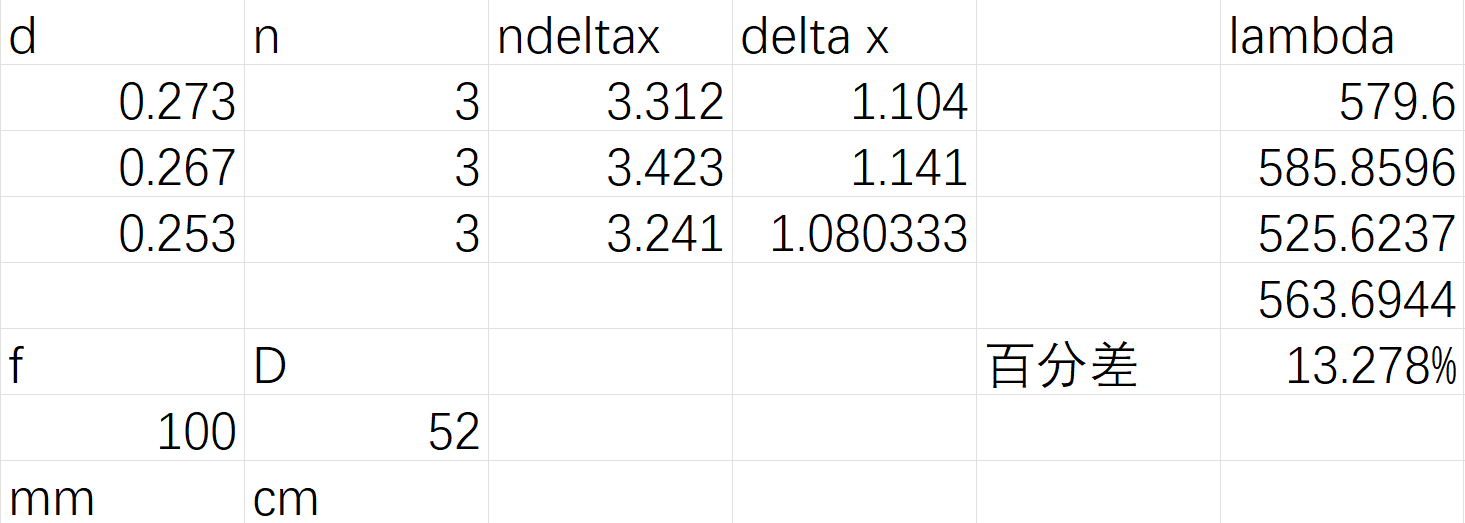
\includegraphics[height=0.3\textheight,width=1\textwidth]{shujvchuli.png}
    \caption{实验数据}\label{shujv}
  \end{figure}
  \subsection{误差分析}
    \subsubsection{$d_{1}$}
    \begin{equation}
      u_{a} = \frac{S(d_{1})}{\sqrt[2]{3}}=8.923\times 10^{-4}\qquad
      u_{b} = \frac{0.001}{\sqrt[2]{3}}=0.0058\qquad
      u_{d_{1}} = 5.87\times 10^{-3}
    \end{equation}

    \subsubsection{$d_{2}$}
    \begin{equation}
      u_{a} = \frac{S(d_{2})}{\sqrt[2]{3}}=2.7\times 10^{-4}\qquad
      u_{b} = \frac{0.001}{\sqrt[2]{3}}=0.0058\qquad
      u_{d_{2}} = 5.827\times 10^{-3}
    \end{equation}

    \subsubsection{$\delta x$}
    \begin{equation}
      u_{a} = \frac{S(\delta x)}{\sqrt[2]{3}}=3.24\times 10^{-4}\qquad
      u_{b} = \frac{0.001}{\sqrt[2]{3}}=0.0058\qquad
      u_{\delta x} = 5.83\times 10^{-3}
    \end{equation}

    \subsubsection{$D$}
    \begin{equation}
      u_{a} = \frac{S(D)}{\sqrt[2]{3}}=5.2\times 10^{-3}\qquad
      u_{b} = \frac{0.01}{\sqrt[2]{3}}=0.058\qquad
      u_{D} = 6.1\times 10^{-3}
    \end{equation}
\section{思考题}
  \subsection{思考题1}
  入射的光线通过双棱镜时,由于双棱镜的形状,光波会被分成两个互相独立的波束。一个波束被折射,另一个波束则通过反射。
  这两个波束分别传播在不同的路径上。
  通过双棱镜的反射和折射,两个波束的光程差会发生变化。这是因为它们在经过不同的光学路径后,会有一定的相位差。
  两个波束再次相遇,它们的相位差会导致干涉现象。如果两个波的相位相同,它们将相干叠加,形成干涉条纹。

  当入射光束在双棱镜上形成等倾角时,两个波束的光程差相对较小,产生的干涉条纹呈直线状,间距均匀。

  波长,间距,双棱镜的折射角,双棱镜的顶角,介质折射率,入射光束的角度。
  \subsection{思考题2} 
  折射角的测量误差通常对实验影响最大。

  精确测量仪器,重复测量,精确调节实验装置,使用窄光源,校正系统误差,考虑温度和湿度。
\newpage

\section{实验中个人的思考与感想}
  \subsection{对于实验个人观点}
  实验中调节实验设备的时候由于设备的差别最终会导致不同设备出现的干涉的条纹不一样,而这种不一样可能是条纹间距特别小,会非常大地程度上
  影响实验最终的结果的测量。

  调节设备的时候花了很多时间进行光路的调直和光具座上仪器的调整高度。但是最后实验得到的干涉条纹的宽度依旧很小,直接使用游标卡尺进行测量
  误差也比较大。

  \subsection{实验中的总结}
  实验中测量了虚光源实相的间距,通过计算得到了虚光源的间距,再通过测量相邻明纹的间隔,最终计算得到光源的波长,和实际值存在一定误差。
\end{document}